\documentclass[titlepage]{article}

\usepackage{frontespizio}

\usepackage[italian]{babel}
\usepackage[utf8x]{inputenc}
\usepackage{amsmath}
\usepackage{graphics}
\usepackage[colorinlistoftodos]{todonotes}
\usepackage{amsmath}
\usepackage{amsfonts}
\usepackage{amssymb}

\begin{document}
\begin{frontespizio}


\Universita {Trento}
\Dipartimento{economia e management}
\Corso [Laurea Magistrale]{Finanza}
\Annoaccademico {2017--2018}
\Logo{logounitn}
\Titoletto {Approfondimenti 2018}
\Titolo {Approccio attuariale alla misurazione del rischio operativo:\\Il Loss Distribution Approach}
\Sottotitolo {LABORATORIO DI SIMULAZIONI FINANZIARIE}
\Candidato [190125]{Erik Holler}
\Candidato [190459]{Elia Scarparo}
\Candidato [190203]{Stefano Zampiero}
\Relatore {Prof.Marco Bee}

\end{frontespizio}
	\newpage

\begin{abstract}
	Descrizione dell'approccio attuariale alla misurazione del rischio operativo utilizzando come metodo il loss distribution approach
\end{abstract}

\section{RISCHIO OPERATIVO: DEFINIZIONE}

\footnote{Fonti: Presentazione PPT del Professor Michele Bonollo dell’Università degli Studi di Padova sul tema: Rischi Operativi e Basilea. Modelli, metodi e problematiche applicative.}Il Comitato di Basilea definisce il rischio operativo come rischio di perdite dovute a inadeguati processi interni, errori umani, carenze nei sistemi operativi o a causa di eventi esterni. \textit{Working paper settembre 2001 –  Comitato di Basilea.} Lo stesso Comitato prevede anche che: ogni banca, nel quadro di una visione integrata e coordinata del risk management, debba maturare una definizione interna di rischi operativi, in funzione del proprio business e dei propri requisiti organizzativi.\\
\footnote{Fonti: Tesi di Laurea Magistrale in Economia e Finanza dell’Università Ca’ Foscari di Venezia del Dott. Giacomo Fasiolo Tozzo. I rischi operativi. A. a. 2014 – 2015.}Il concetto di rischio operativo è dunque intrinseco allo svolgimento di qualsiasi attività umana e per questo correlato ad ogni attività aziendale. Nell’ultimo decennio il sistema bancario e assicurativo è stato interessato da una consapevolezza crescente in merito alla portata strategica dell’attività di gestione e controllo dell’esposizione ai diversi tipi di rischio operativo. Tra i principali fattori che hanno portato a tale consapevolezza devono essere citati: crescita dimensionale delle banche, operazioni di fusione e acquisizione fra banche, massicci investimenti tecnologici attuati da banche, innovazione finanziaria che ha accresciuto la dipendenza da complesse procedure di calcolo e valutazione, sviluppo dei canali telematici, outsourcing.\\
È interessante osservare come sia diffusa l’idea che le perdite operative riguardino prevalentemente aree di business come l’investment banking o il trading su derivati, quando in realtà si riscontrano numerosi esempi di perdite che interessano anche le aree di business più tradizionali. 
\\
Comportamenti infedeli dei dipendenti, business practice improprie, disfunzioni nei sistemi di controllo interno, scarsa trasparenza nella prestazione dei servizi di investimento, sistemi premianti distorti e linee di reporting non chiare sono le evidenze emerse in dissesti finanziari clamorosi, da cui tutti hanno appreso quanto sia importante rafforzare i presidi sul rischio operativo specie in ambito finance e di seguire l’evoluzione di indicatori, anche non finanziari, sull’andamento dell’esposizione al rischio. 
\\
L’emanazione del “Nuovo Accordo sulla Convergenza Internazionale della Misurazione del Capitale e dei coefficienti Patrimoniali”, comunemente detto “Basilea II”, ha fatto in modo che il rischio operativo fosse opportunamente identificato, misurato e monitorato a presidio della solvibilità dell’azienda, con modelli di misurazione del rischio sempre più vicini alle specificità della stessa. È con Basilea 2 che viene esplicitata una definizione in positivo, la circolare n.263 della Banca d’Italia stabilisce che il rischio operativo è, art. 101 Direttiva 2009/139/CE:\\
\textit{“Il rischio di subire perdite derivanti dall’inadeguatezza o dalla disfunzione di procedure, risorse umane e sistemi interni, oppure da eventi esogeni. Nel rischio operativo è compreso il rischio legale, mentre non sono inclusi quelli strategici e di reputazione”. } \newpage
 \footnote{Fonti: Loss Distribution Approach for operational risk, A. Frachot, P. Georges e T. Roncalliy, Groupe de Recherche Operationnelle, Credit Lyonnais, France.}Con riferimento alla classificazione del rischio operativo in categorie di fattori casuali, è possibile introdurre alcuni dettagli, nello specifico il rischio proviene da:
 
\begin{itemize}
\item 	Processi interni: e cioè rischi connessi a ragioni come una formalizzazione inadeguata delle procedure interne, carenze nel sistema di controlli interni ed errori nella definizione e attribuzione di ruoli e responsabilità (progettazione della microstruttura aziendale). In particolare, tale fattore di rischio include eventi relativi a:
\begin{itemize}
\item	Errori nei sistemi di misurazione dei rischi causati da vizi nei modelli o nella formulazione e applicazione delle metodologie (Model Risk);
\item	Errori di contabilizzazione, registrazione e documentazione delle transazioni (Transaction Risk);
\item	Violazioni della sicurezza informatica dovuti a carenze nel sistema dei controlli interni (Security Risk);
\item	Errori nel regolamento di operazioni in titoli e valute con controparti residenti e non; vi rientrano anche insufficienti formalizzazioni delle procedure interne ed errori nella definizione e allocazione di ruoli e responsabilità (Settlement Error).
\end{itemize}
\item	\textbf{Sistemi interni:} si fa riferimento sostanzialmente a problemi di natura tecnica connessi ai sistemi informativi e tecnologici e ai fornitori di public utilities, ovvero connessi alla mancata disponibilità, all’inefficienza, al malfunzionamento o al blocco di hardware, software, telecomunicazioni e information providers.

\item	\textbf{Fattori umani:} ad esempio esistenza di fenomeni di incompetenza, negligenza o mancanza di esperienza del personale addetto, frodi, collusioni e altre attività criminali, violazioni di leggi, normative internazionali, regolamenti interni e standard etici, nonché alla mancanza di una definizione rigorosa e precisa dei ruoli e delle responsabilità. 

\item	\textbf{Eventi esogeni:} si fa normalmente riferimento a situazioni quali gli eventi naturali (terremoti, incendi, inondazioni), politici e militari in grado di influire sul normale svolgimento della gestione aziendale, oltre alle attività criminali.

\footnote{Fonti: Presentazione PPT del Professor Michele Bonollo dell’Università degli Studi di Padova sul tema: Rischi Operativi e Basilea. Modelli, metodi e problematiche applicative.} Il Comitato di Basilea ha previsto poi che il rischio operativo debba essere misurato e gestito con segmentazione dell’attività aziendale, qui si farà riferimento a quella bancaria, sulle diverse linee di business, secondo la seguente classificazione:
 \begin{itemize}
 	

\item	Corporate finance;
\item	Negoziazione e vendite;
\item	Retail banking;
\item	Commercial banking;
\item	Pagamenti e regolamenti;
\item	Gestioni fiduciarie;
\item	Asset management;
\item	Negoziazione al dettaglio.
 \end{itemize}
La normativa di vigilanza Basilea 2 si occupa delle perdite estreme. Il requisito di capitale previsto dalla disciplina è la misura del rischio operativo che deve trovare copertura nel capitale di vigilanza dell’impresa. Non parliamo dunque di perdite attese, le quali trovano già copertura mediante le rettifiche sull’utile di esercizio, esempi: accantonamenti a fondo svalutazione crediti o al fondo rischi su crediti, ma di perdite inattese.
\\

La normativa di vigilanza Basilea 2 si occupa delle perdite estreme. Il requisito di capitale previsto dalla disciplina è la misura del rischio operativo che deve trovare copertura nel capitale di vigilanza dell’impresa. Non parliamo dunque di perdite attese, le quali trovano già copertura mediante le rettifiche sull’utile di esercizio, esempi: accantonamenti a fondo svalutazione crediti o al fondo rischi su crediti, ma di perdite inattese.
\\
	\footnote {Fonti: Loss Distribution Approach for operational risk, A. Frachot, P. Georges e T. Roncalliy, Groupe de Recherche Operationnelle, Credit Lyonnais, France.} La gestione dei rischi operativi si basa sullo sviluppo di due approcci:

\begin{itemize}
\item	\textbf{Qualitativo}: si riferisce a sistemi di controllo tesi a identificare i principali eventi di rischio operativo a cui è esposta l’attività creditizia nei diversi processi e sotto processi e a prevedere una serie di presidi logici, fisici o incorporati nelle procedure che minimizzino la portata di tali eventi in termini di frequenza e gravità del danno economico che potrebbero provocare in caso di concreta manifestazione;

\item	\textbf{Quantitativo:} si riferisce ad un’analisi per il controllo dei rischi operativi su basi statistico-oggettive.
Il Comitato di Basilea ha proposto diverse metodologie per il trattamento prudenziale del rischio operativo, che sono:
\item 	\textbf{Metodo dell’indicatore semplice:} in questo metodo il capitale richiesto nel rispetto del Trattato di Basilea è determinato moltiplicando un indicatore finanziario, come l’utile lordo, per una determinata percentuale – indicatore alpha;

\item		\textbf{Metodo standard:} in questo approccio la banca divide la propria attività in più unità e linee di business standardizzate. All’interno di ciascuna linea di business, la quantità di capitale da accantonare è determinata moltiplicando un indicatore finanziario, come l’utile lordo o la dimensione dell’attivo della data unità per una percentuale fissa (definita fattore beta). Il capitale totale da accantonare è dato dalla somma dei capitali definiti per ciascuna unità o linea di business;

\item		\textbf{Metodo di misurazione interno:} questo approccio fornisce alle banche di usare i propri dati storici di perdita come fattori di input per il calcolo del capitale regolamentare, con modalità definite dall’autorità di vigilanza. Il rischio operativo viene computato come una matrice di rischi di diverso tipo e per diverse linee di business definite dall’autorità di vigilanza, come sopra definite. Il capitale regolamentare è definito all’interno di ciascuna linea di business e per ciascun tipo di perdita moltiplicando la perdita attesa per un determinato fattore gamma. La quantità di capitale regolamentare totale sarà data dalla semplice somma del capitale richiesto per ciascuna linea di business e tipologia di rischio. Il metodo più sofisticato tra quelli di misurazione interna è il Loss Distribution Approach (LDA). Attraverso questo approccio l’impresa stima per ciascuna linea di business / tipologia di rischio la distribuzione di probabilità della severity degli eventi di perdita e della frequency per un certo periodo di tempo. Con queste due distribuzioni, l’impresa computa la distribuzione di probabilità delle perdite operative aggregate. Con il metodo LDA è possibile definire il Capital at Risk, che è la misura di capitale necessaria a coprire le perdite inattese di una determinata business line e per un determinato fattore di rischio oppure per l’impresa nel suo complesso. Il Capital at Risk non è una misura del capitale regolamentare che una banca deve rispettare, ma è senza dubbio utile per l’allocazione di capitale alle diverse business line di cui la banca si compone per calcolarne la reddittività.
\end{itemize}
Il metodo da noi studiato per l’analisi del rischio operativo appartiene alla famiglia dei metodi avanzati di misurazione ed è definito: loss distribution approach e per la sua rappresentazione useremo un orizzonte temporale giornaliero.




\section{LOSS DISTRIBUTION APPROACH}

\footnote{Fonti: Tesi di Laurea Magistrale in Economia e Finanza dell’Università Ca’ Foscari di Venezia del Dott. Giacomo Fasiolo Tozzo. I rischi operativi. A. a. 2014 – 2015.Riferimento preso fino alla definizione dell’art 101 Direttiva 2009/139/CE.}Il \textbf{Loss Distribution Approach – LDA} è il metodo statistico di calcolo considerato più avanzato tra quelli esemplificati come ammissibili dal Comitato di Basilea. Un vantaggio di questo approccio è che la stima delle perdite inattese avviene direttamente e non in modo mediato, ossia tramite l’assunzione di ipotesi circa la possibile relazione esistente tra perdite attese e perdite inattese (che si traduce in un determinato fattore moltiplicativo). L’approccio LDA è di tipo attuariale e due elementi fondamentali sono la frequency (probabilità dell’evento) e la severity (impatto economico dell’evento). Richiamando alla formula da noi usata per la simulazione abbiamo:
\\

$$L =\sum_{i}^{K} X_i$$

dove K $\sim$ Poisson ($\lambda$) e Xi $\sim$ Log$\mathcal{N}($\mu$, $\sigma$^2) (i=1, 2, …, K)
\begin{itemize}


	\item  	Sia Xi \textbf{SEVERITY:} l’impatto economico dell’evento i-esimo nella business line j-esima;
	\item Sia K	\textbf{FREQUENCY:} il numero di eventi di perdita operativa in un orizzonte temporale giornaliero;
	\item Sia  L \textbf{PERDITA:} per l’i-esimo event type all’interno della j-esima business line dell’impresa.
\end{itemize}

Per effettuare il calcolo di indicatori di rischio è necessario determinare o approssimare la distribuzione della variabile casuale perdita (L). Questo richiede di specificare in modo adeguato la famiglia di variabili casuali per il verificarsi di eventi nel tempo (k) e la distribuzione della severity. Nell’approfondimento assegnatoci, abbiamo ricevuto le distribuzioni di tali variabili non definendole partendo dai dati. La distribuzione data della variabile casuale K è una Poissoniana di parametro λ = 5. La distribuzione di severity è invece una Log-normale di parametri mu e sigma specificati per tre diversi casi.\\
\begin{table}[htbp]
\centering
\begin{tabular}{l|r|r}
Caso & Media ($\mu$)& Varianza ($\sigma$^2) \\\hline

1 & 1,5&1 \\
2 & 1,5 &2\\
3 & 3 &1
\end{tabular}
\end{table}


L’impresa può ricavare empiricamente la forma della distribuzione di frequency degli eventi di perdita. Come sopra detto, la frequency degli eventi di perdita nel nostro lavoro è trattata come una variabile casuale di Poisson, che \footnote{Presentazione PPT della Prof.sa Damiana Costanzo dell’Università degli Studi della Calabria. } è una variabile casuale discreta che può assumere qualsiasi valore intero non negativo. È un modello probabilistico adoperato per rappresentare situazioni di conteggio del numero di occorrenze di certi eventi in una unità di tempo o più precisamente il numero di successi in un certo intervallo continuo di tempo nel nostro caso. Una distribuzione di Poisson può derivare, come nel nostro caso, da eventi temporali e cioè dalla ripetizione di un evento in un certo intervallo di tempo, nel nostro caso pari ad una giornata, suddiviso in una serie di intervalli più piccoli. Si assuma che un intervallo sia diviso in un numero molto grande di sottointervalli e che la probabilità del verificarsi di un evento in ogni sottointervallo sia molto piccola. Le ipotesi di base della Poisson sono:
\begin{itemize}
\item la probabilità del verificarsi di un evento è costante per tutti i sottointervalli temporali;
\item l’evento non si può verificare più di una volta in ciascuno dei sottointervalli temporali;
\item eventi che si verificano in intervalli disgiunti sono indipendenti.
\end{itemize}
Distribuzione di Poisson:\\ 

$$p(x)=\frac{\lambda^x}{x!} e^{-\lambda}$ con $0<\lambda <\infty$ dove $X \sim P(\lambda)

\begin{figure}[htbp]
	\centering
	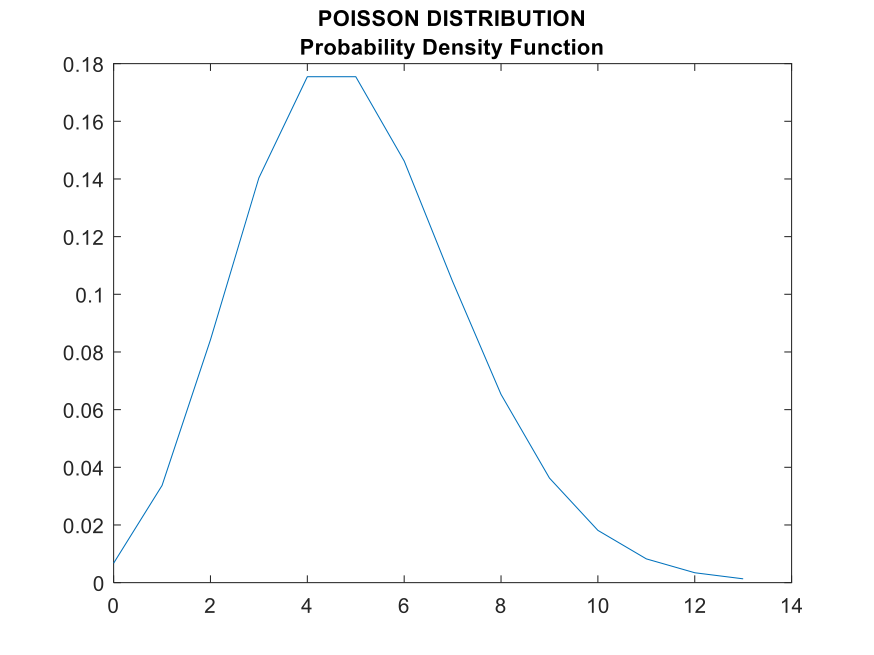
\includegraphics[width=1\textwidth]{poissdistr.png}
	\caption{\label{fig:poissdistr.png}Funzione di densità di probabilità della distribuzione di poisson}
\end{figure}
\\
È possibile dimostrare che: $\text{E}[X_i] = $\lambda$ e  $Var(X) = $\lambda\\

\begin{equation}\label{key}
E(X)=\sum n \frac{\lambda^n}{n!}e^{-\lambda}=\lambda e^{-\lambda} \sum\frac{\lambda^{n-1}}{(n-1)!}=\lambda
\end{equation}

\begin{multline}
 Var(X)=E[X^2]-E[Y]^2
\left\
=\sum n^2 \frac{\lambda^n}{n!}e^{-\lambda}-\lambda^2
\right.\\
\left\
=\sum n(n-1) \frac{\lambda^n}{n!}e^{-\lambda}+\sum n \frac{\lambda^n}{n!}e^{-\lambda}-\lambda^2
\right.\\
\left\
=\lambda^2+\lambda-\lambda^2\right.\\
\left\
=\lambda\\
\right.\\
\end{multline}
La funzione di ripartizione di una Poissoniana indica la probabilità di avere un numero di occorrenze (eventi nell’unità di tempo) inferiore ad una data soglia:\\
\begin{equation}
F(x)=\sum_{i=0}^{x} \frac{\lambda^k \times e^{-\lambda}}{k!}
\end{equation}

Calando la distribuzione di Poisson al nostro elaborato, cerchiamo di spiegarne il funzionamento. A noi è stato dato un certo intervallo temporale, una giornata, lo stesso è stato suddiviso in molteplici sottointervalli temporali della durata di un istante. In ciascuno di questi sottointervalli gli eventi possibili sono due: “si verifica la perdita” e “non si verifica la perdita”. L’evento “si verifica la perdita” viene identificato con un numero 1, l’evento non si verifica la perdita con un numero 0. La distribuzione di Poisson conta gli eventi verificatisi all’interno di ciascun sottointervallo e il numero finale identificato è il numero di perdite che si verificheranno nel corso di una giornata.
\\
La severity – xi (e cioè l’intensità della perdita derivante da una certa tipologia di evento all’interno di una determinata business line) nel nostro modello è andata invece modellizzata con una distribuzione lognormale. Questa distribuzione ammette esclusivamente valori positivi e ha una forma coerente con il dato rappresentato e cioè l’intensità degli eventi di perdita (a severity più basse corrispondono probabilità più alte).  \footnote{Presentazione PPT del Docente: Dott. L. Corain insegnante del Corso di laurea in Ingegneria Civile, Università degli Studi di Padova. Modelli Probabilistici.}La distribuzione lognormale è la distribuzione di probabilità di una variabile aleatoria X il cui logaritmo log(X) segue una distribuzione normale.\\
La funzione di densità di probabilità della distribuzione log-normale è:\\

\begin{equation}\label{key}
F(x)=
\frac{e^{\frac{-(log(x)-\mu)^2}{2\sigma^2}}}{\sqrt{2\pi\sigma^2x}}

\end{equation}

\begin{figure}[htbp]
%	\centering
	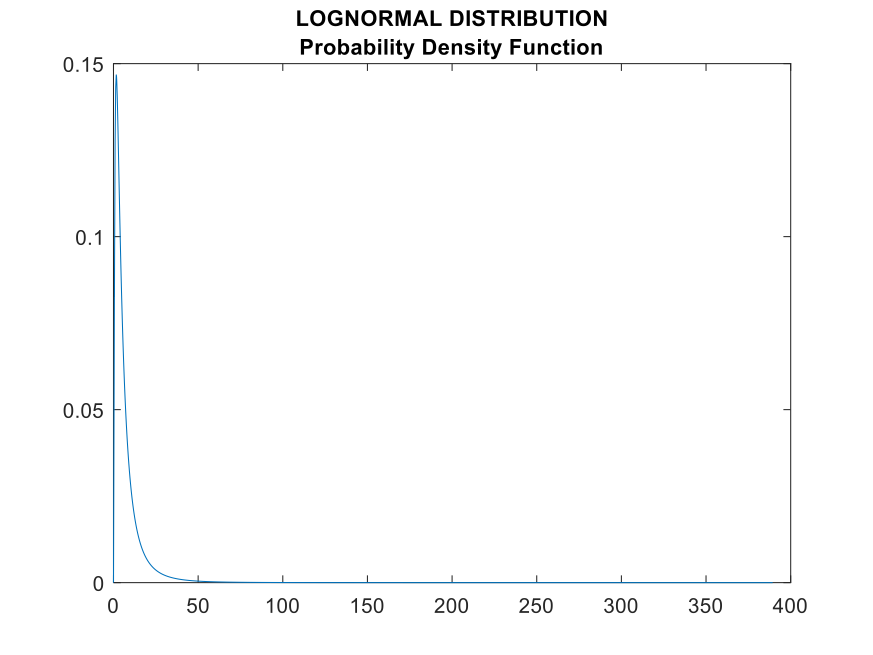
\includegraphics[width=0.9\textwidth]{pdflognormal.png}
	\caption{\label{fig:poissdistr.png}Funzione di densità di probabilità della distribuzione Lognormale}
\end{figure}

 Un aspetto molto importante è la messa a punto di misure di rischio che sintetizzino il rischio di perdite operative e cioè l’incertezza della variabile casuale L. Tra le diverse misure di rischio abbiamo il VAR – Value at Risk. Il VAR si definisce come la massima perdita in un certo intervallo di tempo [t,T] con un dato livello di confidenza (1-α). In caso di variabile casuale continua è dato dal percentile (pari al livello di confidenza) della variabile casuale di perdita L:\\{$VAR=F-1(1-\alpha)
$


\section{MODELLIZZAZIONE DELLA PERDITA E SIMULAZIONE MONTE CARLO}
Una volta che si sono costruite le distribuzioni di severity e di frequency delle perdite operative, è necessario determinare la distribuzione aggregata delle perdite attraverso la convoluzione delle due distribuzioni. Generalmente la determinazione di tale distribuzione attraverso metodi analitici è estremamente complessa, la soluzione più semplice e più diffusa consiste nel ricorrere alla simulazione di Monte Carlo.
\\
\footnote{Fonti: Tesi di Laurea Magistrale in Economia e Finanza dell’Università Ca’ Foscari di Venezia del Dott. Giacomo Fasiolo Tozzo. I rischi operativi. A. a. 2014 – 2015.}Si determinano un sufficiente numero di scenari di frequency e di severity e si costruisce la variabile di perdita operativa L procedendo in questo modo:

\begin{itemize}
\item si genera k attraverso estrazioni casuali dalla distribuzione di frequency;
\item	si generano k variabili xi estratte dalla distribuzione di severity e si effettua la somma per definire L;
\item	si ripete il processo per un numero sufficientemente grande di scenari e si studia la distribuzione empirica delle perdite operative così ottenuta;
\item	dalla distribuzione cumulativa empirica di L si determina il Value at Risk come percentile al livello desiderato.
\end{itemize}
Al fine di definire la distribuzione di frequency abbiamo fatto ricorso alla seguente combinazione di comandi matlab:\\
k = poissrnd(lambda,1,n);
\\

Dove lambda e n sono dati di input che rappresentano rispettivamente media e varianza della distribuzione di Poisson e il numero di estrazioni casuali effettuate dalla distribuzione stessa.
A seguito riportiamo un estratto dell’output della simulazione  
\begin{figure}[htbp]
	%	\centering
	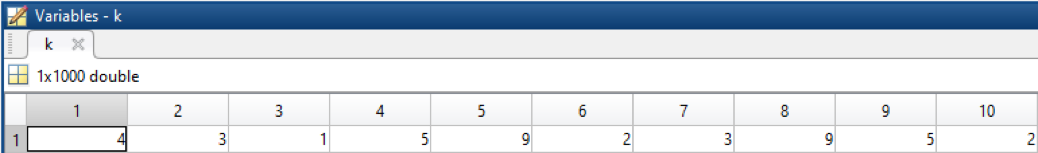
\includegraphics[width=0.9\textwidth]{numeroeventi.png}
	\caption{\label{fig:numeroeventi.png}Estratto dell'output della simulazione }
\end{figure}
Come è possibile notare abbiamo registrato il numero di eventi di perdita all’interno di una giornata per un numero di volte pari ad n = 1.000. Il risultato del nostro lavoro mostra che nella prima simulazione sono state registrate 4 perdite giornaliere, nella seconda simulazione 3 eventi di perdita giornalieri e così via. Si riporta di seguito una rappresentazione grafica della frequency, nonché il codice Matlab, commentato nei vari passaggi, necessario ad ottenerla:
\\
\begin{itemize}
\item	Calcoliamo i valori di massimo e di minimo di k
\\
max=max(k);
\\
min=min(k);
\\
\item	Definiamo i valori contenuti tra il minimo ed il massimo di k con uno spazio unitario tra un valore e l'altro
\\
edges = min:1:max;
\\
\item	Contiamo i valori contenuti in edges che si osservano nel vettore k \\
m= histc(k,edges);
\\
\item Costruiamo il grafico a barre contenente i valori di frequency
\\
bar(edges,m);
\\
\end{itemize}
\begin{figure}[htbp]
	\centering
	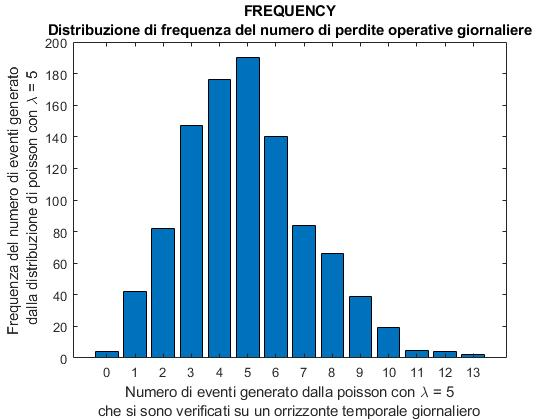
\includegraphics[width=0.9\textwidth]{FREQUENCY.jpg}
	\caption{\label{fig:frog}Distribuzione di frequency.}
\end{figure}
La distribuzione rappresentata della variabile discreta K, presenta elevate frequenze per valori prossimi al valore medio definito nei dati come da consegna (λ=5), mentre si possono notare frequenze sempre minori per valori lontani da λ.
\\
Il passo successivo ci richiede di definire la severity; ciò è stato fatto attraverso estrazioni casuali da una distribuzione lognormale con parametri µ e σ. Il numero di estrazioni di severity di volta in volta dipende dall’i-esimo valore di K definito al passaggio precedente. Dunque, riprendendo i valori prima scritti, il numero di estrazioni effettuate per la prima simulazione è pari a 4 mentre per la seconda è pari a 3 e cosi via.
\\
x(1:k(i),s)=lognrnd(mu(p),sigma(p),k(i),1);
\begin{itemize}
\item x è la matrice composta dalle estrazioni di severity dove ogni colonna rappresenta una simulazione delle intensità dei k eventi di perdita;
\item k(i)rappresenta l’i-esimo valore di frequenza degli eventi di perdita;
\item s è un contatore del numero di simulazioni 
\item mu(p),sigma(p)rappresentano i parametri della distribuzione log-normale
\item k(i),1 all’interno della funzione lognrnd rappresentano le dimensioni del vettore simulato
\end{itemize}
\\
Il terzo passaggio richiede di effettuare la simulazione n volte al fine di giungere alla distribuzione di perdita operativa L. Implementiamo ciò tramite un ciclo che calcoli le perdite operative sulla base di valori casuali trovati al passaggio precedente. Operativamente i valori di ogni colonna della matrice x, vengono sommati calcolando così la perdita L legata all'i-esimo event type e alla j-esima business line. I valori di severity sono simulati per tre diversi scenari, abbiamo dunque tre matrici di severity diverse. Per ciascuna si effettua la computazione di perdita operativa.
\\

for p=1:3
\\
for i=1:n
\\
x(1:k(i),s)=lognrnd(mu(p),sigma(p),k(i),1);
\\
s=s+1;     
\\
if s==n+1
\\
s=1;
\\
break
\\
end
\\
end
\\
L(p,:)=sum(x); 
\\
Lsort(p,:)=sort(L(p,:));
\\
 var(p)=quantile(Lsort(p,:),alpha);
\\
end
\\

Riportiamo di seguito un estratto di una matrice di severity. L’estratto in questione è relativo al terzo caso, questo perché il ciclo for dopo aver definito la matrice severity relativa al primo caso e dunque calcolato su di essa la distribuzione di perdita L e calcolato il VaR, riparte da capo ridefinendo la matrice di severity. Questa sovrascrive quella del primo caso e così la matrice di severity definita nel terzo caso sostituisce quella del secondo caso. Ciò significa che tra gli oggetti nel workspace ad ogni run dello script risulterà esclusivamente la tabella di severity dell’ultimo caso simulato. Attenzione perché il numero di elementi in ciascuna colonna è definito da k, che rimane uguale per tutti i casi, dunque ciò che cambia da una matrice di severity e l’altra è solo il valore degli elementi non nulli.
\\
\begin{figure}[top]
	\centering
	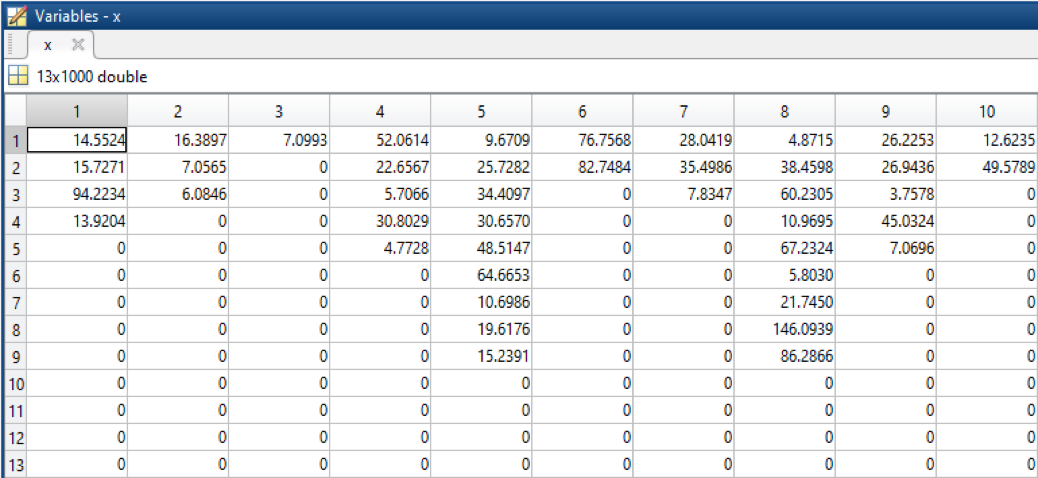
\includegraphics[width=0.9\textwidth]{severity.png}
	\caption{\label{fig:severity.png}Una parte della matrice x}
\end{figure}
\\
Consci del fatto che la funzione quantile ordinerebbe automaticamente i valori di perdita per il calcolo del Var, abbiamo preferito creare una matrice ordinata delle perdite operative (Lsort) tramite la funzione sort che ci permette quindi di verificare l’eventuale presenza e peso di outliers nel vettore L.\\



\begin{figure}[htbp]
	\centering
	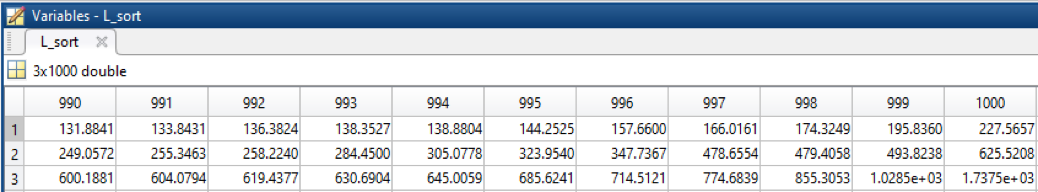
\includegraphics[width=0.9\textwidth]{losss.png}
	\caption{\label{fig:losss.png}utlimi 10 quantili della distribuzione ordinata delle perdite operative}
\end{figure}
\\
Il comando Lvar(p)=quantile(Lsort(p,:),alpha) ci permette di espletare il quarto punto della simulazione Montecarlo e cioè il calcolo del Var al 99° percentile rappresentato da alpha. Nello specifico sono stati individuati i Var per tre diversi scenari. 
\\

Riportiamo di seguito i tre diversi casi:
\begin{figure}[htbp]
	\centering
	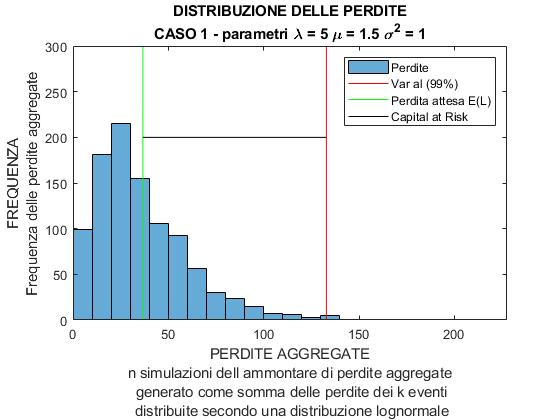
\includegraphics[width=0.9\textwidth]{LOSS1.jpg}
	\caption{\label{fig:losss.png}distribuzione delle perdite operative aggragate:caso 1}
\end{figure}
\begin{figure}[htbp]
	\centering
	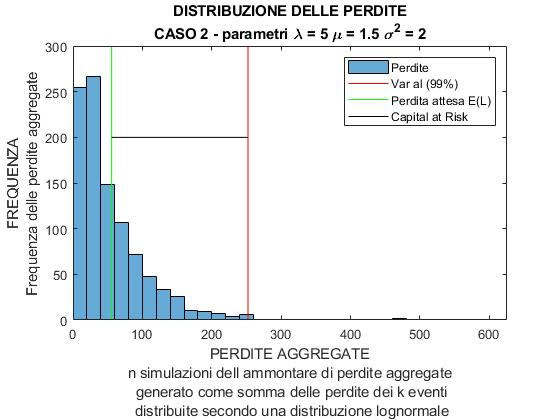
\includegraphics[width=0.9\textwidth]{LOSS2.jpg}
	\caption{\label{fig:losss.png}distribuzione delle perdite operative aggragate:caso 2}
\end{figure}
\begin{figure}[htbp]
	\centering
	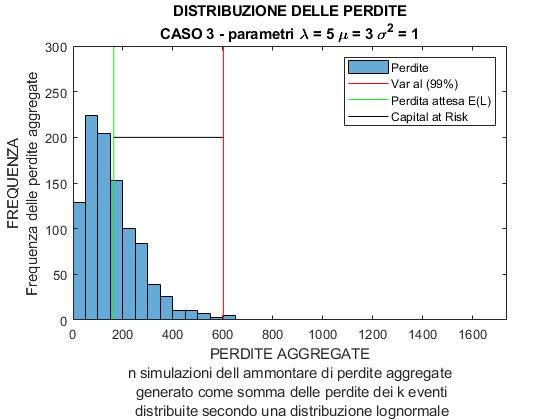
\includegraphics[width=0.9\textwidth]{LOSS3.jpg}
	\caption{\label{fig:losss.png}distribuzione delle perdite operative aggragate:caso 3}
\end{figure}
Procediamo ad effettuare il confronto fra i 3 diversi casi rispetto ai seguenti parametri:
\begin{itemize}
\item 	Valore atteso di perdita E(L);
\item 	Value at Risk al 99%.
\end{itemize}
\begin{table}[htbp]
	\centering
	\begin{tabular}{l|rrr}
		Caso n-esimo & Value at Risk & Expected Loss& Capital at Risk \\\hline
		\\
		1 & 132,8636&36,6176&96,2459 \\
		2 & 252,2018 &55,7423&196,4595\\
		3 & 602,1337 &163,1085&439,0252
	\end{tabular}
\end{table}
Confrontando il caso 1 e il caso 2, il parametro di distinzione è la varianza della distribuzione di severity che è rispettivamente pari ad 1 e a 2, tutti gli altri parametri sono uguali. Dunque, nel caso 2 ci aspettiamo una maggiore dispersione dei valori di severity rispetto alla media. Infatti, lo conferma il Capital at Risk (Capital at Risk = Value at Risk – Expected Loss) che nel caso 2 è pari a 196,4595 mentre nel caso 1 è pari a 96,2459. Il valore di Expected Loss è simile tra i due casi, nel secondo è di poco superiore (55,7423 vs 36,6176).
\\
Confrontando il caso 1 con il caso 3, il parametro di distinzione è la media della distribuzione di severity che è rispettivamente pari a 1 e a 3, gli altri parametri sono uguali. Nel caso 3 troviamo un Capital at Risk molto superiore rispetto al caso 1, con una differenza di 342,7793. Il valore di perdita attesa nel caso 3 è sensibilmente superiore rispetto al caso 1, rispettivamente pari a 163,1085 e 36,6176.
\\
Confrontando il caso 2 con il caso 3, i parametri di distinzione sono la varianza, rispettivamente pari a 2 e a 1 e la media, rispettivamente pari a 1,5 e a 3, delle distribuzioni di severity, gli altri parametri sono uguali. Nel caso 2 troviamo un CaR inferiore rispetto al caso 3, rispettivamente pari a 196,4595 e 439,0252. Nel caso 2 inoltre il valore di perdita attesa è inferiore rispetto al caso 3 con una differenza di 107,3662.
\\
Dall’analisi comparativa effettuata possiamo trarre che ad una maggiore media della distribuzione di severity segue un maggior valore atteso della distribuzione di perdita operativa (L). Ad una maggiore varianza della distribuzione di severity invece corrisponde un maggiore Capital at Risk. L’aumento della media della distribuzione di severity ha un impatto direttamente proporzionale sulla scala della distribuzione di perdita operativa e questo si riflette quindi sulle code della distribuzione influenzando Value at risk e Capital at Risk; questo effetto pare essere superiore a quello dovuto alla varianza. Questo perché, come nel caso 3, nonostante una varianza pari alla metà di quella del caso 2, abbiamo un Capital at Risk superiore rispetto al caso 2. Ciò è dovuto ad una media della distribuzione di severity del caso 3 doppia rispetto a quella del caso 2.
\\
Il lavoro qui svolto poggia su determinate ipotesi, che qui ricapitoliamo:
\begin{itemize}

\item 	gli eventi di perdita devono essere reciprocamente indipendenti;
\item 	il costo di ogni “incidente” deve essere identicamente distribuito;
\item 	la distribuzione di frequency e quella di severity devono essere indipendenti.
	
\end{itemize}
Ricapitolando, la simulazione Montecarlo sceglie casualmente un numero giornaliero di eventi dalla distribuzione di frequency. La scelta più probabile sarà sempre uguale alla media, in questo caso pari a λ. Questo numero scelto casualmente è la frequenza per quell’iterazione. La frequenza viene quindi utilizzata come numero di estrazioni che la simulazione Monte Carlo selezionerà dalla distribuzione di severity. Ognuna di queste estrazioni dalla distribuzione di severity rappresenta un evento di perdita. Tutti gli importi di perdita ottenuti vengono sommati per creare la quantità giornaliera di perdita complessiva. Questo processo viene ripetuto fino a quando viene eseguito il numero desiderato di iterazioni. Gli importi delle perdite complessivi di ogni iterazione sono ordinati dal più piccolo al più grande, e la media di tutti i risultati è la perdita attesa della distribuzione di perdita aggregata.
\\
L'importo del Value at Risk per la determinata tipologia di evento e all’interno della prespecificata linea di business è dato dal Xo (es. 99.99o, 99o, 95°) percentile della distribuzione di perdita aggregata e rappresenta la perdita aggregata corrispondente a quel determinato percentile, che l’intermediario potrebbe subire entro un determinato orizzonte temporale, giornaliero o annuale che sia. L’approccio del VaR (Value at Risk) rappresenta una metodologia di quantificazione dell’esposizione di un intermediario finanziario alle diverse tipologie di rischio e di determinazione dell’ammontare di capitale proprio necessario ad assorbire perdite potenziali conseguenti a tali rischi. Il VaR esprime la massima perdita che può essere conseguita in un determinato periodo di tempo nel (1 - $\alpha$) degli eventi, dove il coefficiente α rappresenta il livello di tolleranza.
\\

\begin{figure}[htbp]
	\centering
	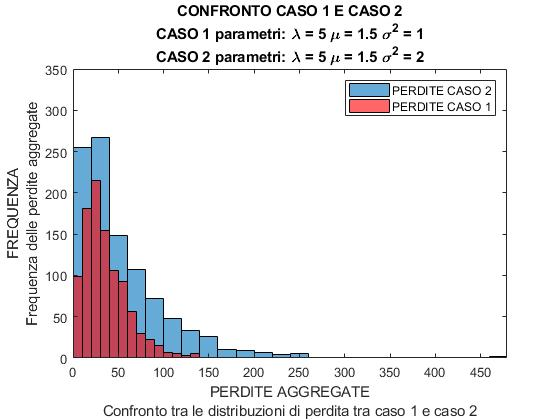
\includegraphics[width=0.9\textwidth]{1VS2.jpg}
	\caption{\label{fig:losss.png}Confronto tra le distribuzioni di perdita di caso 1 e caso 2}
\end{figure}
\begin{figure}[htbp]
	\centering
	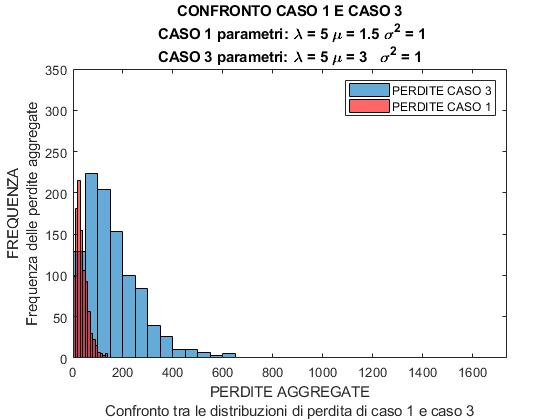
\includegraphics[width=0.9\textwidth]{1VS3.jpg}
	\caption{\label{fig:losss.png}Confronto tra le distribuzioni di perdita di caso 1 e caso 3}
\end{figure}
\begin{figure}[htbp]
	\centering
	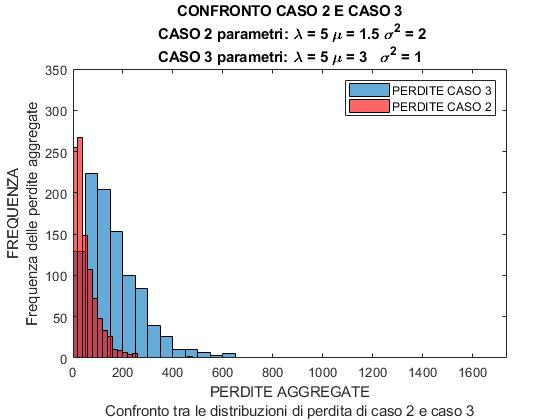
\includegraphics[width=0.9\textwidth]{2VS3.jpg}
	\caption{\label{fig:losss.png}confronto tra le distribuzioni di perdita di caso 2 e caso 3}
\end{figure}
\section{AGGREGAZIONE DELLE CLASSI DI RISCHIO CAPITAL AT RISK}
Ora disponiamo delle distribuzioni (empiriche) delle perdite aggregate giornaliere per ogni classe di rischio ed unità di business. \footnote{Fonti: Tesi di Laurea Magistrale in Economia e Finanza dell’Università Ca’ Foscari di Venezia del Dott. Giacomo Fasiolo Tozzo. I rischi operativi. A. a. 2014 – 2015.} Il calcolo del Value at Risk complessivo a fronte del rischio operativo può essere effettuato semplicemente sommando i requisiti di capitale determinati per ciascuna business line e tipologia di evento. In questo modo si assume una correlazione lineare nulla tra ogni coppia di event type.\\

L’alternativa, prevista anche dall’ accordo di Basilea, acconsente l’utilizzo di altre tecniche di aggregazione, assumendo strutture di correlazione diverse. Viene riconosciuta la possibilità alle banche, di considerare eventuali correlazioni esistenti tra le perdite di natura operativa delle diverse business line e quelle derivanti dalle varie tipologie di evento, a condizione che possano dimostrare all’autorità di vigilanza, con un elevato grado di certezza, che le metodologie usate per stimare la correlazione siano robuste, integre e capaci di riflettere l’incertezza che tipicamente caratterizza tali stime nei periodi di stress.
\\
\footnote{Fonti: Loss Distribution Approach for operational risk; A. Frachot P. Georges e T.Roncalliy Groupe de Recherche Operationnelle, Credit Lyonnais, France.}La stessa procedura di aggregazione vista per il Value at Risk può essere utilizzata per il Capital at Risk. Il Capital at Risk è la differenza tra il Value at Risk e l’Expected Loss per l’ente. Questa misura è interpretabile come capitale che l’ente dovrebbe accantonare per coprire la perdita inattesa. Non è un requisito obbligatorio per la regolamentazione attuale, ma è senza dubbio un fattore che incrementerebbe la solidità patrimoniale dell’organizzazione.
\\
Noi abbiamo calcolato il CaR all’interno di una sola business line in riferimento ad un solo event type, ma tale approccio può essere esteso in termini aggregati tenendo conto di n-event type su n-business line con gli opportuni adattamenti. 
Vediamo dunque uno schema per il calcolo del Capital at Risk aggregato per un’impresa con una successiva allocazione del capitale medesimo a ciascuna business line:
\begin{itemize}


	\item 	Computazione del Capital at Risk per ciascuna Business Line e per ciacuna tipologia di rischio;
	\item Calcolo del Capital at Risk totale tenendo in considerazione di eventuali effetti mitigatori della diversificazione di capitale;
	\item 	Allocazione di componenti di Capital at Risk aggregato a ciascun event type;
	\item 	Allocazione di componenti di ciascuna quantità di capitale definita al punto 3, considerando eventuali effetti mitigatori, a ciascuna unità di business.
\end{itemize}
\begin{table}[htbp]
	\centering
	\begin{tabular}{l|rrr}
		Caso n-esimo & Value at Risk & Expected Loss& Capital at Risk \\\hline
		\\
		1 & 132,8636&36,6176&96,2459 \\
		2 & 252,2018 &55,7423&196,4595\\
		3 & 602,1337 &163,1085&439,0252
	\end{tabular}
\end{table}
\newpage
Portando l’attenzione ai risultati trovati, evidenziamo che:
\\

		Dal confronto del primo e del secondo caso, il CaR è superiore in quest’ultimo. Dunque, un aumento della varianza della distribuzione di severity comporta un maggiore capitale occorrente alla copertura delle perdite inattese. Questo è dovuto al fatto che, a parità di impatti economici di perdita, la coda della seconda distribuzione di perdita è più pesante rispetto a quella della prima distribuzione ed aumenta così l’ammontare delle possibili perdite estreme. Presentiamo il grafico a riguardo per una più facile comprensione del fenomeno:



\begin{figure}[htbp]
	\centering
	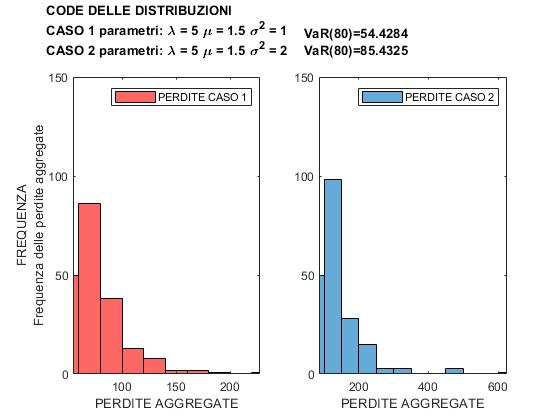
\includegraphics[width=0.8\textwidth]{CODE 1VS2.jpg}
	\caption{\label{fig:CODE 1VS2.jpg}Code delle distribuzioni di perdita caso 1 e caso 2}
\end{figure}
	Analizzando il primo e il terzo caso, si nota che il CaR è sensibilmente superiore in quest’ultimo caso con una differenza pari a 242,566. L’aumento della media della distribuzione di severity comporta un incremento dell’impatto economico dei singoli eventi di perdita, che, se aggregati, portano a una distribuzione di perdita operativa su scala maggiore. Gli effetti si possono notare dal confronto delle code delle distribuzioni nei due casi, che sottolineano una differente pesantezza sugli stessi valori aggregati di perdite:
\begin{figure}[htbp]
	\centering
	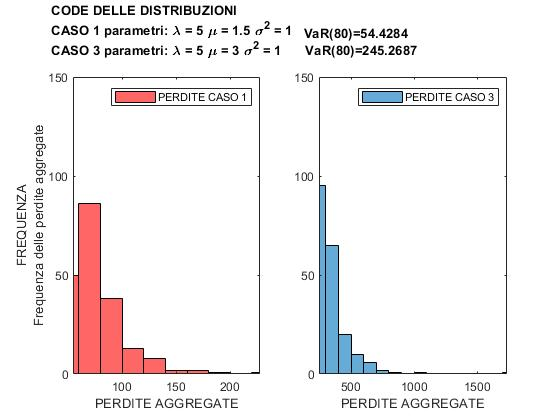
\includegraphics[width=0.7\textwidth]{CODE1VS3.jpg}
	\caption{\label{fig:CODE 1VS3.jpg}Code delle distribuzioni di perdita caso 1 e caso 3}
\end{figure}

		Al variare di entrambi i parametri della distribuzione di severity, osservabile nel confronto tra caso due e caso tre, si nota un maggior CaR in quest’ultimo caso. L’aspetto interessante è che la variazione dei parametri è inversa. Da questa analisi quindi, l’aumento del CaR ci suggerisce che l’effetto dell’aumento della media della distribuzione di severity è più impattante rispetto a quello di riduzione della varianza. Riportiamo a seguito il confronto delle code delle due distribuzioni:
\begin{figure}[htbp]
	\centering
	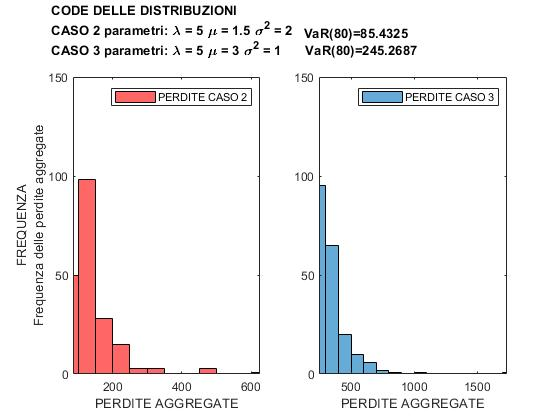
\includegraphics[width=0.8\textwidth]{CODE2VS3.jpg}
	\caption{\label{fig:CODE 2VS3.jpg}Code delle distribuzioni di perdita caso 2 e caso 3}
\end{figure}
\newpage
\section{DEFINIZIONE DELLE DISTRIBUZIONI DI FREQUENCY E SEVERITY}
 I dati sono una risorsa fondamentale per la gestione del rischio operativo, questi potrebbero essere di difficile reperimento o di bassa qualità, in concreto possono riscontrarsi problemi di:
 \begin{itemize}
 	

\item Mancanza di dati per alcune business line e tipologie di evento;
\item 	I dati interni possono essere distorti verso perdite di basso ammontare. Eventi estremi possono essere difficilmente presenti nei database interni;
\item 	Potrebbero essere registrate perdite solo sopra una determinata soglia. Questo potrebbe dare origine a delle distribuzioni troncate e portare ad una sovrastima della severity;
\item 	Dati eventualmente reperiti all’esterno dell’ente potrebbero essere distorti. Una giusta combinazione tra dati interni ed esterni è necessaria al fine di un buon lavoro di analisi. 
 \end{itemize}
Ci potremmo dunque chiedere quale potrebbe essere la migliore distribuzione per la severity of loss partendo dai dati. Assumiamo di avere un insieme di probability density function (PDF). Qual è la migliore distribuzione di questo set per descrivere la distribuzione di severity delle perdite? Prima di tutto occorre definire l’insieme delle PDF, tra le quali individueremo la distribuzione migliore per approssimare i dati. Dopodiché, dobbiamo definire un criterio di scelta della distribuzione. A questo fine potremmo ricorrere ad un Q-Q plot. Per questa via si prenderà come distribuzione dei dati di severity quella i cui quantili approssimano al meglio i quantili della distribuzione empirica.  Il Q-Q plot è uno strumento grafico che confronta i quantili della distribuzione empirica con i quantili della distribuzione teorica di riferimento. Se la distribuzione empirica è ben approssimata da quella teorica, i quantili empirici dovrebbero essere simili ai quantili “teorici” dello stesso livello q. Dunque, in un grafico a dispersione che rappresenti sulle ascisse i quantili empirici e sulle ordinate i quantili teorici della distribuzione di riferimento, i punti dovrebbero disporsi lungo la bisettrice del secondo quadrante. 
\\
Nel nostro caso abbiamo tratto i valori di severity of loss da una distribuzione Log-normale già definita in partenza. Avendo un numero di osservazioni empiriche tratto da una poissoniana di parametro pari a cinque, e per cui limitato, non riteniamo opportuno rappresentare graficamente il Q-Q plot per la verifica della distribuzione teorica.\\
Per quanto riguarda la distribuzione di frequency delle perdite, generalmente si usa una variabile casuale con distribuzione di Poisson. Il grafico rappresentato di seguito riporta:
\begin{itemize}
	\item i quantili della distribuzione empirica costruita a partire dalle osservazioni casuali tratte dalla distribuzione di Poisson con parametro $\lambda$=5;
	\item 	i quantili della distribuzione di Poisson teorica con parametro $\lambda$=5
\end{itemize}
Com’è possibile notare la distribuzione teorica approssima bene quella empirica, questo perché le osservazioni di frequency da noi usate non sono basate su dati reali ma sono valori casuali tratti dalla distribuzione teorica stessa.
Se i quantili della distribuzione empirica non si posizionassero in prossimità della bisettrice del secondo quadrante allora la distribuzione teorica non rappresenterebbe bene quella empirica. Occorrerebbe quindi ripetere l’analisi con altre distribuzioni teoriche.
\begin{figure}[htbp]
	\centering
	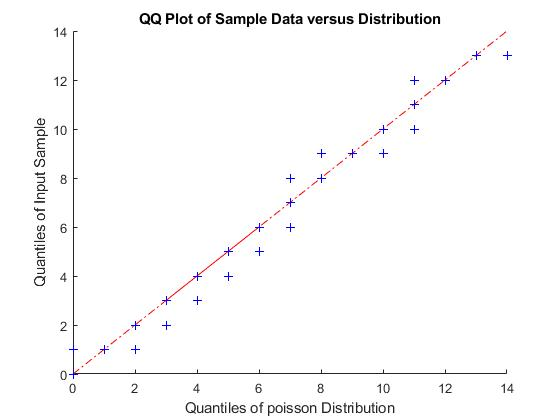
\includegraphics[width=0.9\textwidth]{QQPLOT.jpg}
	\caption{\label{fig:losss.png}QQ plot}
\end{figure}
Un altro modo per verificare la compatibilità tra distribuzioni di frequency empirica e teorica scelta è calcolare media e varianza della prima. Se questi due parametri hanno valori simili allora la distribuzione empirica sarà ben approssimata da una Poissoniana. Se invece sono sensibilmente diversi si opterà per una distribuzione Binomiale negativa. Questo ragionamento si basa sulla caratteristica di egual media e varianza della distribuzione di Poisson come sopra dimostrato.
\newpage
\newpage
\section{VANTAGGI E LIMITI DEL LOSS DISTRIBUTION APPROACH}
Distribution Approach” presenta numerosi vantaggi, tra i quali: 
\begin{itemize}


	\item 	I risultati si basano sulle caratteristiche specifiche di ogni singola istituzione, invece di basarsi su una proxy o su una media di settore. Anche se le aziende operano in diverse linea di attività, ogni impresa ha un proprio profilo di rischio specifico. 

	\item 	I risultati si basano su principi matematici simili a quelli utilizzati per la stima del requisito patrimoniale per il rischio di mercato e per il rischio di credito. L'approccio LDA può specificare un orizzonte temporale e un livello di confidenza. Di conseguenza, i tre tipi di capitale di rischio possono essere combinati in maniera statisticamente valida. 

	\item 	La separazione tra frequency e severity favorisce la precisione nella stima e la comprensione del processo di generazione del rischio. 

	\item 	L’utilizzo di distribuzioni statistiche ben conosciute può aiutare il processo di calibrazione. 

	\item 	Si tratta di modelli abbastanza flessibili e adattabili a nuovi business operativi, inoltre richiede una potenza computazionale limitata.
\end{itemize}
	 Tuttavia, l'approccio LDA presenta anche alcune limitazioni: 
	\begin{itemize}
	\item 	È un modello ad alta intensità di dati. Questo è forse il più grande problema del “Loss Distribution Approach”. Per applicare questo metodo in modo coerente in tutta l'organizzazione, è necessaria una serie di dati completa riguardante gli eventi di perdita. 

	\item La calibrazione necessita di un vasto campione statistico strutturato e qualitativamente adeguato, l’integrazione di dati interni, dati esterni, analisi di scenario e talvolta del giudizio di esperti può essere difficoltosa. 

	\item 	L’assunzione di indipendenza tra la distribuzione di frequency e quella di severity costituisce un grosso limite. 

	\item 	L’approccio presuppone la stabilità del sistema, il modello è poco rappresentativo se il processo di rischio sottostante è fortemente dinamico. 
\end{itemize}
In riferimento al nostro approfondimento l’indicatore di rischio usato è il Var al 99\%. Il grosso limite del VaR è legato al fatto che si stima soltanto la massima perdita probabile per un determinato intervallo di confidenza, tralasciando così eventuali eventi estremi che invece sono quelli più rilevanti dal punto di vista delle perdite che essi possono causare. Per tale motivo si ha il rischio di considerare uguali, cioè caratterizzati dallo stesso VaR, distribuzioni di perdita che presentano un comportamento nelle code estremamente diverso. Per evitare di sottostimare le perdite eccedenti il VaR stesso, si può ricorrere al $Expected shortfall\alpha\%$ \\  Conditional Value at Risk dato dal valore atteso delle perdite che superano il Var
$ES\alpha\%=E(L|L>VAR\alpha%)
$.




\newpage
\begin{thebibliography}{9}
	\bibitem{pantieri:arte}
	Pantieri, Lorenzo e Tommaso Gordini (2017),
	\emph{Loss Distribution Approach for operational risk},
	\url{http://www.lorenzopantieri.net/LaTeX_files/ArteLaTeX.pdf}.
		\bibitem{pantieri:arte}
	Pantieri, Lorenzo e Tommaso Gordini (2017),
	\emph{Loss Distribution Approach for operational risk},
	\url{http://www.lorenzopantieri.net/LaTeX_files/ArteLaTeX.pdf}.
		\bibitem{pantieri:arte}
	Pantieri, Lorenzo e Tommaso Gordini (2017),
	\emph{Loss Distribution Approach for operational risk},
	\url{http://www.lorenzopantieri.net/LaTeX_files/ArteLaTeX.pdf}.
		\bibitem{pantieri:arte}
	Pantieri, Lorenzo e Tommaso Gordini (2017),
	\emph{Loss Distribution Approach for operational risk},
	\url{http://www.lorenzopantieri.net/LaTeX_files/ArteLaTeX.pdf}.
	Loss Distribution Approach for operational risk, A. Frachot, P. Georges & T. Roncalliy, Groupe de Recherche Operationnelle, Credit Lyonnais, France 
\\
	[Wiley Series in Probability and Statistics] Klugman, S.A. and Panjer, H.H. and Wilmt, G.E. – Loss Models_From Data to Desicions, 2012
\\
	Presentazione PPT del Professor Michele Bonollo dell’Università degli Studi di Padova sul tema: Rischi Operativi e Basilea 2. Modelli, metodi e problematiche applicative. Link web: http://slideplayer.it/slide/537049/ ;
\\
	Presentazione PPT della Professoressa Simona Cosma dell’Università del Salento sul tema: Il calcolo del VAR operativo mediante la metodologia stocastica parametrica. Link web:\\ http://docplayer.it/35191968-Il-calcolo-del-var-operativo-mediante-la-metodologia-stocastica-parametrica-simona-cosma.html
	Lezione n. 5. - 28/3/03. Università degli Studi di Roma Tre, sezione di Matematica. Dipartimento di Matematica e Fisica. Link web: http://www.mat.uniroma3.it/didattica_interattiva/aa_-02_03/st1/lez5.pdf 
\\
	Tesi di Laurea Magistrale del Dott. Giacomo Fasiolo Tozzo. Corso di Laurea: Economia e Finanza presso l’Università Ca’ Foscari di Venezia. Relatore: prof. Andrea Giacomelli. Anno accademico 2014 – 2015. Titolo della tesi: I Rischi Operativi. Link web:\\ http://dspace.unive.it/bitstream/handle/10579/6862/832502-1190252.pdf?sequence=2 .
	Presentazione PPT della Prof.sa Damiana Costanzo dell’Università degli Studi della Calabria. Link web: \\ http://www.ecostat.unical.it/Costanzo/Didattica/Probabilit%C3%A0%20ed%20-Inferenza%20Statistica/lucidi_10.pdf . 
	Presentazione PPT del Docente: Dott. L. Corain insegnante del Corso di laurea in Ingegneria Civile, Università degli Studi di Padova. Modelli Probabilistici. Link web: http://static.gest.unipd.it/~livio/PDF/PDF_CIVILE/Modelli%20probabilistici.pdf .
	
\end{thebibliography}


\end{document}